\chapter{関連研究}
\label{chap:kanren}

本章では関連研究を紹介し、それらの特徴や本研究との関連性について示す。

\newpage

メモを含めて手書きデータの活用を目的とする先行研究は数多く存在する。

\section{主要な研究領域}
手書きメモ・イラストに関する主要な研究領域を解説する。

\section{手書きメモ支援システム}
タブレットやPDA等のデバイスを用いて手書きメモの作成や運用を効率化する研究が行われている。

\subsection{Notepal}
Davisらが提案するNotepal\cite{Davis1999NotePalsLN}(図\ref{notepal})はPalm Pilot等のPDAを用いて手書きメモをグループで共有可能にするシステムである。
他のマシンからもメモを閲覧できるようにクレードルでホストマシンと接続した際にデータを共有スペースにアップロードする。
これにより個人のメモを他のメンバーが参照し、組織的に活用することを可能にした。
またPDAの限られた画面面積では入力しづらいケースに対応するためデジタルペンによって描かれた紙のデータも共有することができる。
一方で手書きストロークの中にリンクを埋めこむ等の機能はないためメモ同士をリンクさせるといった活用はできない。

\begin{figure}[H]
    \centering
    \fbox{ 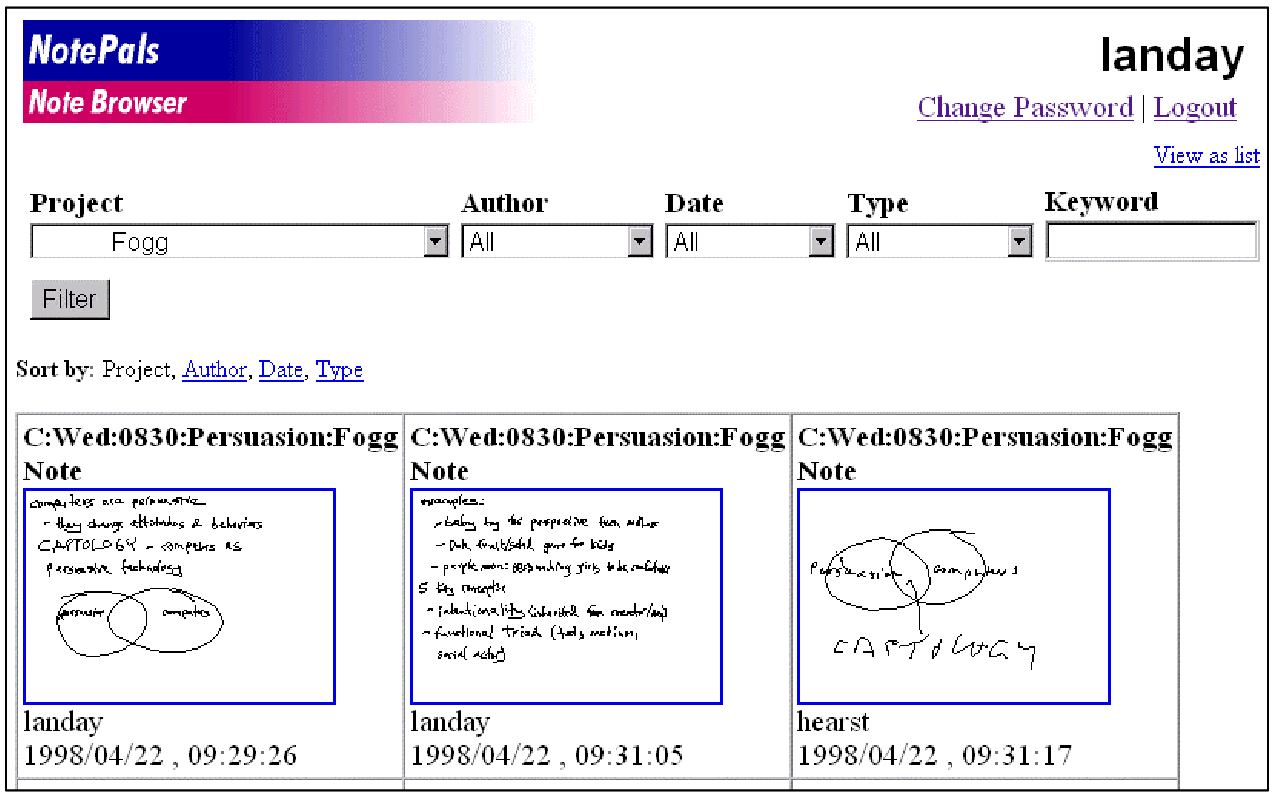
\includegraphics[width=10cm]{images/notepal.png} }
    \caption{Notepalの画面}
    \label{notepal}
\end{figure}

%\subsection{InkAnchor}
%\begin{figure}[H]
%    \centering
%    \fbox {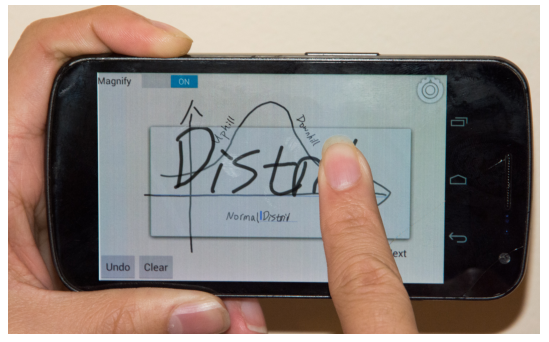
\includegraphics[width=10cm]{images/inkanchor.png}}
%    \caption{InkAnchorの画面}
%    \label{inkanchor}
%\end{figure}
%PDAやスマートフォン等の画面の小さい端末はタブレットなどに比べて手書き入力が比較的困難になる傾向にある。
%RenらによるInkAnchor\cite{Ren2014InkAnchorEI}(図\ref{inkanchor})では指を用いて小型の端末に手書きメモを入力するケースに役立つ、
%テキストエリアと独立した手書き入力エリア等のインターフェースが提案されている。

\subsection{InkSeine}
Hinckleyらによって開発されたInkSeine\cite{Hinckley2007InkSeineIS}(図\ref{inkseine})はペンインターフェースを備えたタブレットPCを主眼に置いた電子スクラップブックシステムである。
キーボードは使わずにペンのみで操作が完結するようUIが設計されており、テキスト入力も手書き文字認識によって行う。
また入力した手書き文字をファイルやWebページの検索に活用したり、検索結果のスナップショットをハイパーリンクと共にキャンバスに貼り付ける等の機能を備えている。
一方でスクラップブックをタブレットデバイス上で再現することを目的としているため、共同編集等の活用法は想定されていない。

\begin{figure}[H]
    \centering
    \fbox{ 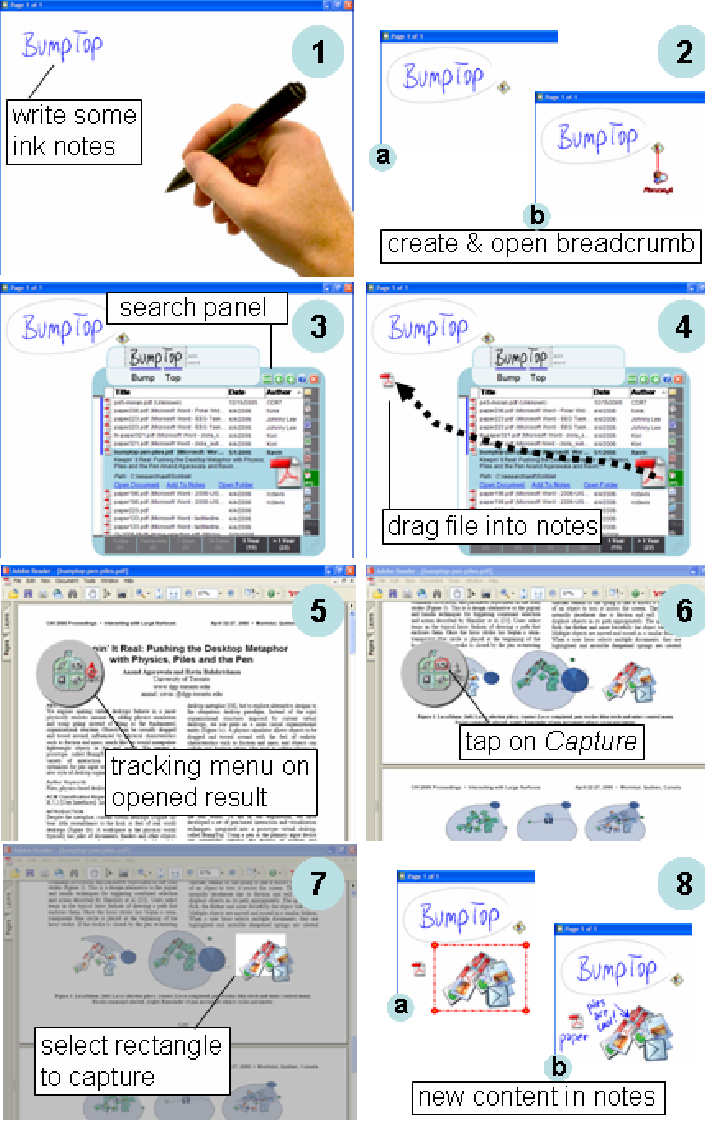
\includegraphics[width=10cm]{images/inkseine.png} }
    \caption{InkSeineの操作画面}
    \label{inkseine}
\end{figure}

\section{デザイン・プロトタイピングツール}
アプリケーションやWebサイトのUIを設計する際スケッチがよく利用される\cite{Newman2000SitemapsSA}。
スケッチとしての手書きデータをデザインやプロトタイピングに取り入れる試みとして以下の研究が挙げられる。

\subsection{DENIM}

\begin{figure}[H] \begin{minipage}{0.5\hsize}
                         \begin{center} \fbox {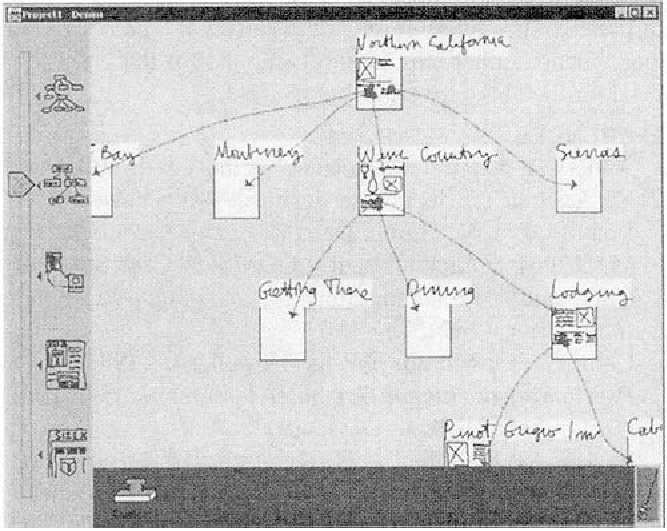
\includegraphics[width=70mm]{images/denim1.png}}
                         \end{center} \caption{DENIMの画面} \label{fig:denim1}
\end{minipage} \begin{minipage}{0.5\hsize}
                   \begin{center} \fbox {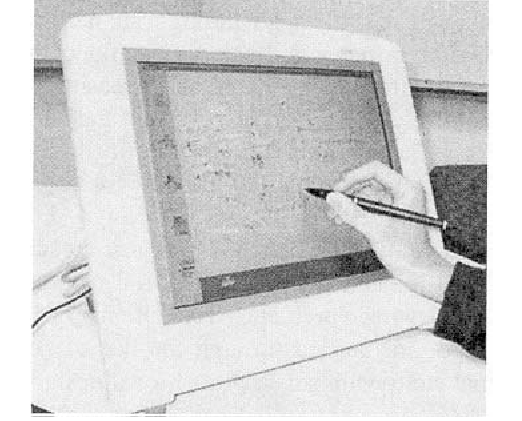
\includegraphics[width=70mm]{images/denim2.png}}
                   \end{center} \caption{操作を行うタブレット機器} \label{fig:denim2}
\end{minipage}
\end{figure}

Linらはタブレットからのスケッチを元にWebサイトのデザインやナビゲーションの設計の支援を行うシステムDENIMを開発した\cite{Lin2000DENIMFA}(図\ref{fig:denim1})。
図\ref{fig:denim2}のようなタブレット機器から操作できるように設計されている。
手書き入力だけでなくWebサイトのディテールから大まかな画面遷移に至るまでをカバーするためにスケッチを行うキャンバスにはズーミングインターフェースが備わっている。


\subsection{SILK}

\begin{figure}[H]
    \centering
    \fbox{ 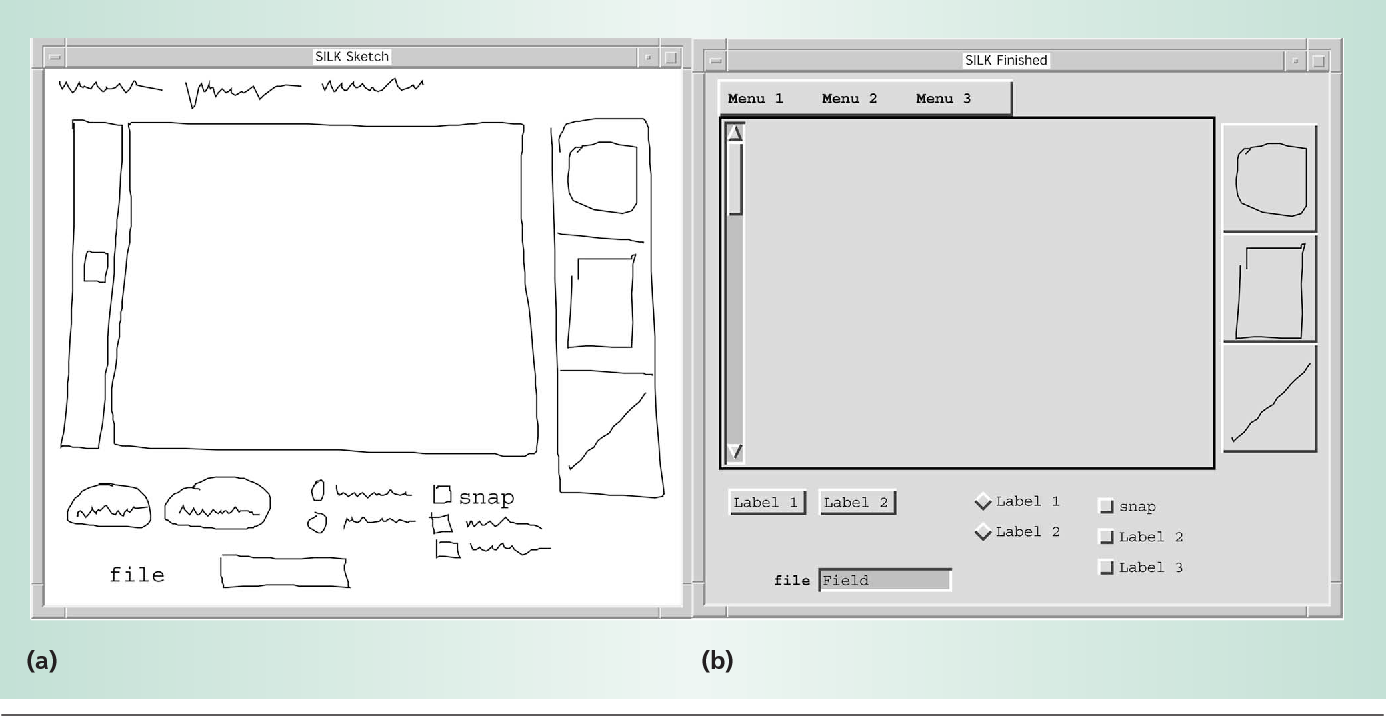
\includegraphics[width=10cm]{images/silk.png} }
    \caption{SILKの画面}
    \label{fig:silk}
\end{figure}

Landayらはスタイラスから入力した手書きデータから実際に動作するGUIを構築するSILK(Sketching Interfaces Like Krazy)というシステムを実装した
\cite{Landay2001SketchingIT}(図\ref{fig:silk})。
GUIを設計する際は紙にアイデアをスケッチすることが一般的だったがこのシステムでは手書きのスケッチを元に実際に動作するプロトタイプを作成することができる。

\subsection{IntaractivePaper}
\begin{figure}[H]
    \centering
    \fbox{ 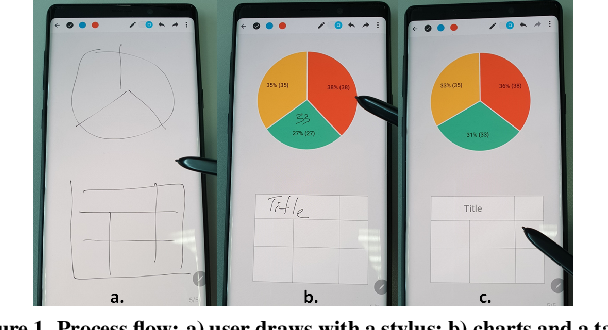
\includegraphics[width=10cm]{images/interactivepaper.png} }
    \caption{IntaractivePaperの画面}
    \label{fig:intaractivepaper}
\end{figure}
ZhelezniakovらによるIntaractivePaper\cite{Zhelezniakov2019InteractivePaperMI}ではラフな手書きストロークからパイチャートやテーブル等の要素に変換する機能を備えている。
またモバイル機器から利用できるように認識フローや選択インターフェースが再検討されている(図\ref{fig:intaractivepaper})。

\section{手書きデータを利用したActive Readingやコラボレーション}
Active Readingや共同作業を行う場合にも手書き入力は頻繁に活用される。

\subsection{XLibris}
\begin{figure}[H]
    \centering
    \fbox{ 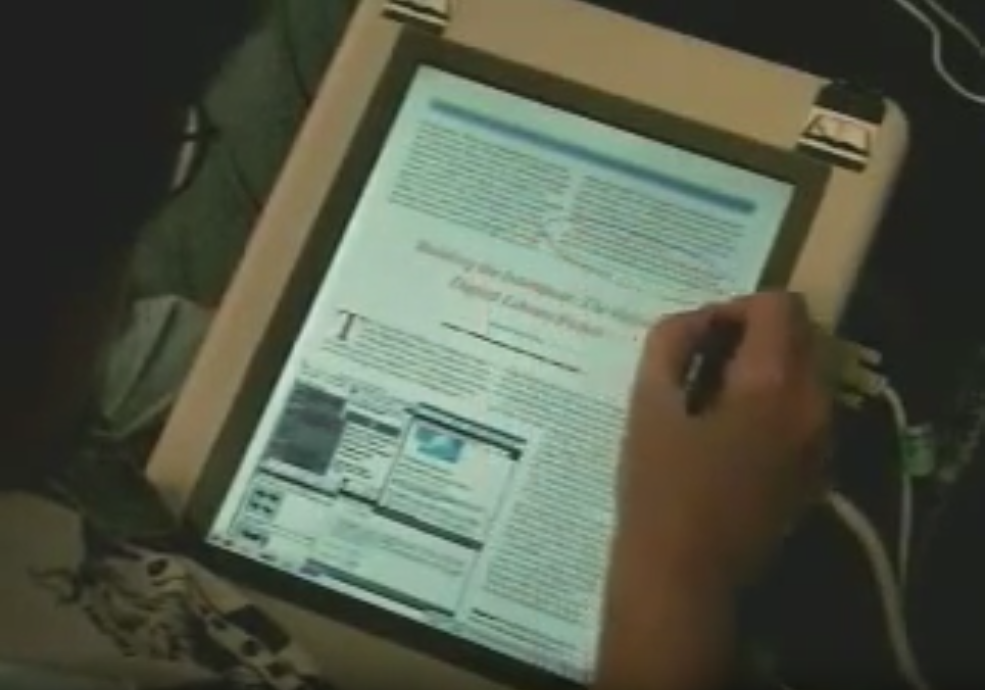
\includegraphics[width=10cm]{images/xlibris.png} }
    \caption{操作中のXLibris}
    \label{fig:xlibris}
\end{figure}
PriceらによるXLibris\cite{Price1998XLibrisTA}はタブレットデバイス上でActive Readingを行うことを目的としたシステムである。
手書きによる注釈やハイライトの入力や、入力したページを一覧画面から参照する機能等を備えている(図\ref{fig:xlibris})。
Active Readingをタブレットデバイスで再現することを主眼に置いているため、文書の脇に追記する注釈以上の、
自在な手書きメモやイラストを書き加えるという用途は想定されていない。

%\subsection{Sensing Tablet Grasp + Micro-mobility for Active Reading}
%
%\begin{figure}[H] \begin{minipage}{0.5\hsize}
%                      \begin{center} \fbox {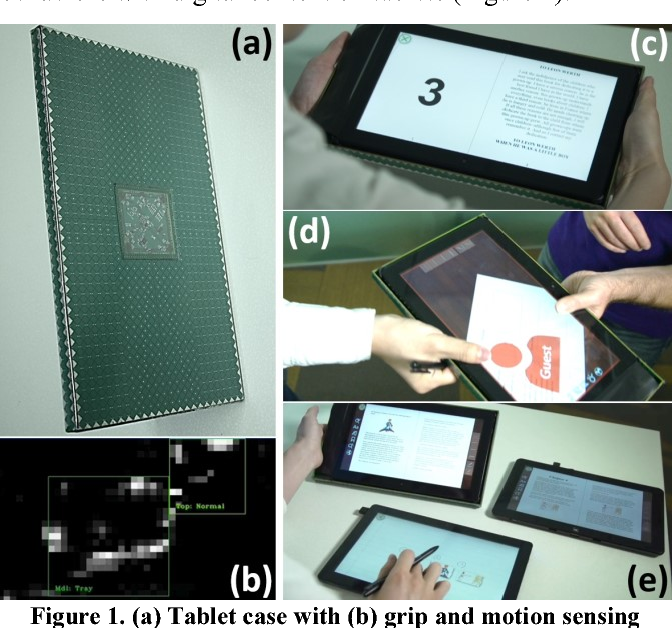
\includegraphics[width=70mm]{images/grasp1.png}}
%                      \end{center} \caption{} \label{fig:grasp1}
%\end{minipage} \begin{minipage}{0.5\hsize}
%                   \begin{center} \fbox {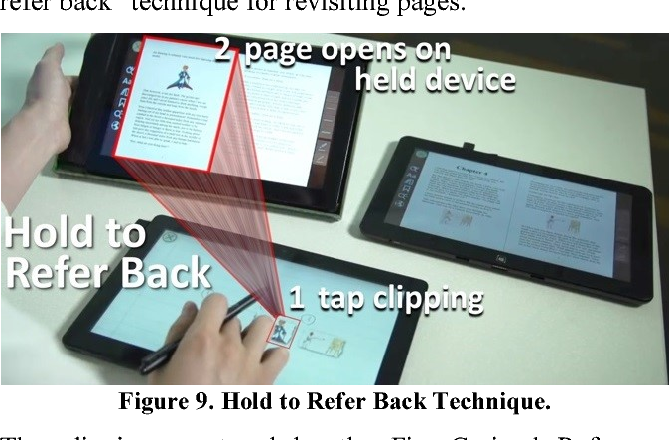
\includegraphics[width=70mm]{images/grasp2.png}}
%                   \end{center} \caption{} \label{fig:grasp2}
%\end{minipage}
%\end{figure}
%
%Yoonらは共同でアクティブリーディングを行う際に生じるMicro-mobilityというコンテンツの再配置や方向づけをデバイスでセンシングすることで
%単一のデバイスによる共同作業や、複数デバイス間の相互参照をサポートするシステムを提案した\cite{Yoon2015SensingTG}。

\subsection{SketchComm}

\begin{figure}[H] \begin{minipage}{0.5\hsize}
                      \begin{center} \fbox {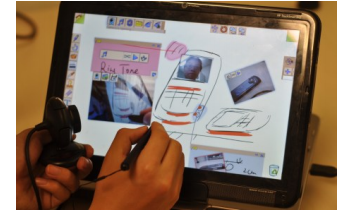
\includegraphics[width=70mm]{images/sketchcomm1.png}}
                      \end{center} \caption{} \label{fig:sketchcomm1}
\end{minipage} \begin{minipage}{0.5\hsize}
                   \begin{center} \fbox {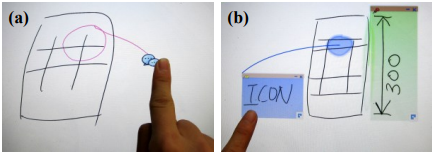
\includegraphics[width=70mm]{images/sketchcomm2.png}}
                   \end{center} \caption{} \label{fig:sketchcomm2}
\end{minipage}
\end{figure}
LiらによるSketchComm\cite{Li2012SketchCommAT}はアイデアに関するスケッチが非同期的にレビューされることを念頭に置いて設計されたシステムである(図\ref{fig:sketchcomm1})。
対面によるリアルタイムのコミュニケーションと異なりコンテキストが欠落しないよう、注釈やコメント、音声データ等をスケッチの内部に埋め込むことができる(図\ref{fig:sketchcomm2})。
SketchCommはコラボレーションツールではあるものの、CreatorとReviewerという役割を持ったユーザー同士という特殊な状況に特化しているため
Wikiのようなカジュアルな共同編集は想定されていない。